% DOCUMENT SETUP
\documentclass[letterpaper,11pt,twoside]{article}
\hyphenpenalty=8000
\textwidth=125mm
\textheight=200mm
\usepackage[top=3cm, bottom=3cm, inner=3cm, outer=3cm, includehead]{geometry}
\usepackage{fancyhdr}
\setlength{\headheight}{13.6pt} % Fix for fancyhdr warning
\addtolength{\topmargin}{-1.6pt} % Optional: further fix as suggested
\pagestyle{fancy}
\fancyhead{}
\fancyfoot{}
\raggedbottom
\usepackage{xurl}
\usepackage{graphicx}
\usepackage{amssymb}
\usepackage{mathtools}
\usepackage{alltt}
\usepackage{amsmath}
\usepackage[hidelinks, pdftex]{hyperref}
\urlstyle{same}
\usepackage[T1]{fontenc}
\usepackage[utf8]{inputenc}
\usepackage{lmodern}
\usepackage{csquotes}
\usepackage[notes, backend=biber]{biblatex-chicago}
\pagenumbering{arabic}
\setcounter{page}{1}
\graphicspath{{./imgs/}}
\usepackage[english]{babel}
%\usepackage[french]{babel}
%\usepackage[spanish]{babel}

% AUTHOR AND TITLE
\begin{document}
\fancyhead[RO]{ELEC 475 Lab 1, Alistair Barfoot and Luke Barry\ \ \ \ \thepage}
\begin{center}
    \LARGE
    \textbf{ELEC 475 Lab 1, Alistair Barfoot and Luke Barry}\\[12pt]
    \normalsize
\end{center}

\section{Model Details}
% This section should contain all details of the network, sufficient to recreate the model. This could be in textual form, diagrammatic, or other. The main requirement is that the description has sufficient details to fully and exactly recreate the model
The model used for this lab was an simple Multi-Layer Perceptron (MLP) autoencoder. This network takes in an image, encodes it using the model, and then decodes it. The resultant image is a compressed version of the original image.
\\
\\
MLP consists of a network of artificial neurons organized in layers and connected between layers via a learnable weight. In the case of the encoder, there is one neuron for each pixel in the input image (in this case, that would be 28x28=784). At each layer, the amount of neurons halves until reaching the final value known as the "bottleneck number". This model used a bottleneck number of 8.
\\
\\
In the case of the decoder, the same process is used, but in reverse. The number of artificial neurons starts at the bottleneck number, doubling at each layer until reaching enough neurons for each pixel in the image.

\section{Training Details}
% This section should include all details of the training, sufficient to exactly reproduce the training. This should include the optimization method used (e.g. SGD, Adam, etc.), optimization hyperparameters (e.g. initial learning rate, momentum, etc.), any learning rate scheduling used, and all other relevant details.
We trained our model on the MNIST dataset, a set of 60,000 images of white handwritten digits on a black background, each 28x28 pixels in size. 
\\
\\
For the training process, we used an Adam optimizer with a learning rate of 10e-3 and a weight decay of 10e-5. The model was trained with a batch size of 2048 and for 50 epochs down to a bottleneck size of 8. To calculate the loss, we used the Mean Squared Error (MSE) equation which computes as follows.
\begin{equation}
  MSE = \frac{1}{n} \sum_{i=1}^{n}(Y_i - \hat{Y}_i)^2
\end{equation}
\\
Where: \\
$n$ \>\> is the number of data points \\
$Y_i$ \> is the observed value\\
$\hat{Y}_i$ \> is the predicted value \\
\\
\\
In this case, the observed and predicted values are each individual pixel value within the image.

\section{Results}
The loss curve for the training process as outlined is shown below.\\
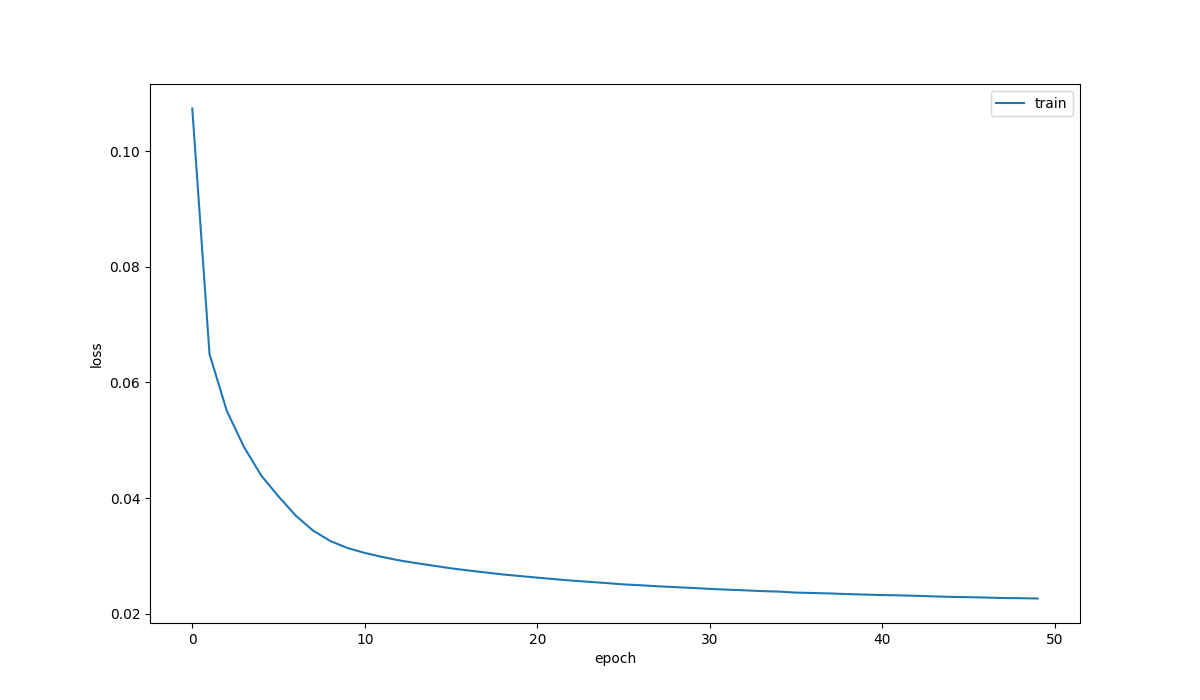
\includegraphics[scale=0.45]{src/loss.MLP.8.png}
\\
The loss for the first epoch is pretty high, over 10\%. In the first few epochs, however, the loss drops signifiantly until around epoch 20 where the loss remains at about 3\%. Overall, the curve follows a logarithmic pattern where most of the loss is reduced in the first few epochs. As the number of epochs increases, each epoch has less of an impact to the training of the model.
\\
\\
This is an indicator of a successful training process and it leads to suggest that the model is trained well.
\end{document}